\documentclass[11pt,a4paper]{article}

\usepackage{amsmath}  
\usepackage{amsfonts} 
\usepackage{graphicx}
\graphicspath{ {./images/} }
%\usepackage[demo]{graphicx}
\usepackage[usenames]{color}
\usepackage{mathtools}
\usepackage{algorithm}
\usepackage[noend]{algpseudocode}
\usepackage{float}
\usepackage{xcolor}


\DeclarePairedDelimiter{\abs}{\lvert}{\rvert}
\DeclareMathOperator{\esssupp}{ess\,supp}


 \textwidth=16cm \hoffset = -1.9cm
 \lineskip=1.5\lineskip


% MATH -----------------------------------------------------------
\newcommand{\Real}{\mathbb R}
\newcommand{\eps}{\varepsilon}
\newcommand{\diag}{\mathrm{diag}}
\newcommand{\nbr}{\mathrm{nbr}}
\newcommand{\F}{\mathcal{F}}
\newcommand{\Hil}{\mathscr{H}}
\newcommand{\LL}{\mathcal{L}}
\newcommand{\G}{\mathscr{G}}
\newcommand{\s}{\mathbb{S}}
\newcommand{\p}{\mathscr{P}}
\newcommand{\C}{\mathscr{C}}
\newcommand{\one}[1]{\mathbf{1}_{\{#1\}}}
\newcommand{\oneset}[1]{\mathbf{1}_{#1}}
\renewcommand{\P}{\mathbb{P}}
\newcommand{\Q}{\mathsf{Q}}
\newcommand{\E}{\mathbb{E}}
\newcommand{\osimplex}{\mathcal{S}^{d-1}}
\newcommand{\csimplex}{\bar{\mathcal{S}}^{d-1}}
\newcommand{\argmin}{\mathrm{argmin}}
\newcommand{\argmax}{\mathrm{argmax}}
\newcommand{\var}{\mathrm{Var}}
\newcommand{\cov}{\mathrm{Cov}}
\newcommand{\ind}{\mathrm{I}}
\newcommand{\D}{\mathscr{D}}
\newcommand{\Borel}{\mathscr{B}}
\newcommand{\M}{\mathcal{M}}
\newcommand{\Z}{\mathcal{Z}}
\renewcommand{\d}[1]{\ensuremath{\operatorname{d}\!{#1}}}

\newcommand{\ben}{\begin{enumerate}}
\newcommand{\een}{\end{enumerate}}
\newcommand{\ds}{\displaystyle}

\DeclareMathOperator{\trace}{tr}
\DeclareMathOperator*{\esssup}{ess~sup}
\DeclareMathOperator*{\essinf}{ess~inf}
\DeclareMathOperator*{\diam}{diam}
\DeclareMathOperator*{\ROC}{ROC}
\DeclareMathOperator*{\sinc}{sinc}
\DeclareMathOperator*{\sign}{sign}
\newcommand{\voila}{\hfill $\blacksquare$}
\newcommand{\Id}{\mathrm{Id}}
\newcommand{\K}{\mathbb{K}}
\renewcommand{\Re}{\mathrm{Re}}
\renewcommand{\vec}[1]{\mathbf{#1}}
\newcommand*\diff{\mathop{}\!\mathrm{d}}




\title{Fire Ants Model and Method}

\begin{document}
 \maketitle

\section{The Model}

We are proposing a new model for the RIFA invasion based on a self-exciting point process.

In this new approach we are seeking to simplify and improve on Keith and Spring agent-based model \cite{Keith} with the aim to reduce the running time without compromising on flexibility and completeness.

The model of Keith and Spring focused on reconstructing the historical trajectory of the invasion to determine if the current eradication strategy was successful. Their method consisted of constructing a likelihood model in terms of some unknown parameters that included, among other things, the phylogeny, jump type, founding type and treatment success rate. They then constructed the dependencies among the known and unknown parameters and defined all conditional distributions.

The posterior distribution was then sampled using a generalised Gibbs technique that enables transdimensional sampling, which is used when the number of parameters is unknown, as in their case.

A key feature of our model is that it will not need to include the phylogeny of the nests in the likelihood, which will result in a much lower computational time when running the inference code. This will also allow the model to be adapted to other type of invasions where control strategies will have to be decided rapidly as new data is acquired. {\color{red}The phylogeny can however be reintroduced in cases where this would be useful. VVV we can perhaps add an explanation on how this can be done below?}.

We have been also considering the detection processes in parallel with the founding events in a similar way as in Jewell's model for infectious diseases \cite{Jewell}. We then included unobserved nests alongside observed nests in the detection likelihood to fully model the missing data. Finally, the model is designed to considered events happening continuously in time.

Let us consider a self-exciting spatial-temporal point process $N$ as a generalization of an Hawkes model {\color{red} \cite{Hawkes71}}. We can then specify an intensity function $\lambda(x, y, t)$ which represents the infinitesimal expected  rate of events at time $t$ and location $(x, y)$  given all the events up to time $t$.

Here $\mathcal{F}$ is a $\sigma$-algebra on $S \times [0, \infty )$, where $S$ is a bounded region of $\mathbb{R}^2$ and $[0, \infty)$ is the time interval. $N(A)$ is a counting measure $N: \mathcal{F} \to \mathbb{R}$ representing the number of points in $A$ for $A \in \mathcal{F}$.

We will consider $N$ to be an inhomogeneous Poisson process, for which $\lambda(x, y, f)$ is deterministic, i.e. depends only on $(x, y)$ and $f$ \cite{Shoenberg} {\color{red}VVV I am not sure this is correct. If N is a Poison process and $\lambda$ is deterministic we would not have a self exciting point process which depends on the history of all events up to time $t$. I think it is the background process that is a Poisson process with rate $\mu$ and it is the likelihood of the process that is that of an inhomogeneous Poisson process while N is a random counting measure (a stationary point process)}. The function $g(x - x', y - y', f - f')$ is the clustering density, where $f'$ are the times of founding of parents nests and the spatial coordinates $(x', y')$ will specify the location $s'$ of a parent nest.

We can then write the intensity function for new nests, {\color{red} conditional over the past history of the process $\mathcal{H}_t$}, in term of a stochastic integral:

\[
\lambda(x, y, t {\color{red}| \mathcal{H}_t}) = \mu(x, y, t) + \int_{0}^{t} \iint_{S} g(x - x', y - y', f - f') \d N(x', y', f')
\]
were $\d N(x', y', f') = 1$ if the infinitesimal element $\d N(x', y', f')$ contains a parent and is 0 otherwise. $\lambda(x, y, t)$ may be thought of as the frequency with which events are expected to occur around a particular location $(x, y, t)$ in space–time.

in our model, we consider the temporal behavior of the process as independent of the spatial behavior so we can write

\[
\lambda(x, y, t {\color{red}| \mathcal{H}_t}) = \mu(x, y, t) + \int_{0}^{t} \iint_{S} m(f-f') \cdot l((x - x'), (y - y')) \d N(x', y', f')
\]
where $\mu$ is a background term, while $m$ and $l$ are the triggering functions for time and space respectively. {\color{red} From now on we will omit the explicit conditioning on the past history $\mathcal{H}_t$ for ease of notation.}

New individuals from the invasive species can be introduced at any time by carriers like animals or humans. For simplicity, in the RIFA invasion we will assume that these exogenous introductions are not happening. Also we assume to know time and location of the first nest.  We will therefore set the background term $\mu(x, y, f) $ equal to 0. {\color{red} VVV We will need to introduce a term for the jumps inside the intensity function (L\'evi distribution):
\begin{equation*}
  p(x; \nu, c ) = \sqrt{\frac{c}{2\pi}} \frac{e^{-\frac{c}{2(x-\nu)}}}{(x - \nu)^{3/2}}  
\end{equation*}
were $\nu$ is the location parameter and $c$ is the scale parameter).}

Each parent nest will be able to found more than one nest, with the number of nests founded per nest per month being a parameter $\zeta$, therefore the temporal triggering kernel will be a step function. Also the nest will have a maturation time $t_m$ of 8 months. Before this time they will not be able to produce new nests. 

The step function will be:


\[
m (f - f') =
\begin{cases}
0, & \mbox{if} \quad f - f' < t_{m} \\
\zeta, & \mbox{if} \quad f - f' \geq t_{m}
\end{cases}
\]
where $f$ is the founding time of the new nest and $f'$ is the founding time of the parent nest.

For the newly founded nests we will consider a radial distance from the parent nest with an exponential distribution. The distribution over the angular direction will be uniform as it is equally possible to found a nest in every direction from the parent nest.

\begin{equation}
l(x - x', y - y')= J \bigg(\frac{1}{2 \pi} \sigma e^{- \sigma r}\bigg)
\end{equation}
where $J$ is the Jacobian

\[
J =  
\begin{vmatrix}
	\frac{\partial r}{\partial x} & \frac{\partial r}{\partial y} \\
	\frac{\partial \theta}{\partial x} & \frac{\partial \theta}{\partial y} \\
\end{vmatrix}
\]
where

\[
r^{2} = (x - x')^{2} + (y - y')^{2}
\]
and

\[
\theta = tan^{-1} \Bigg [\frac{y - y'}{x - x'} \Bigg ]
\]
therefore

\[
J = \frac{1}{\sqrt{(x - x')^{2} + (y - y')^{2}}}.
\]
We also make the assumption that nests are killed as soon as they are detected, so we introduce an indicator function $I(t' - t)$ such that

\[
I (t' - t) =
\begin{cases}
1, & \mbox{if} \quad t' -  t> 0 \\
0, & \mbox{otherwise}
\end{cases}
\]
where $t'$ represents the time of detection. So the conditional intensity function will be

\[
\lambda(x, y, t, f) = \int_{0}^{t} \int_{0}^{f} \iint_{S} m(f - f') \cdot I(t' - t)\cdot \frac{\sigma J }{2 \pi} e^{- \sigma r} \d N(x',y',t',f')
\]
where now the term $\d N(x',y',t',f')$ is 1 if a nest was founded in an infinitesimal time about $f'$ at a location in an infinitesimal region about $(x', y')$ and was detected in an infinitesimal time around $t'$ and is $0$ otherwise. Note that we must have $\d N(x',y',t',f')=0$ whenever $f' \geq t'$.

{\color{red} Equivalently, since N is a counting measure, we can write

\[
\lambda(x, y, t, f) = \sum_{ k: t_k < t } m(f - f_k) \cdot I(t_k - t)\cdot \frac{\sigma}{2 \pi} \frac{1}{\sqrt{(x - x_k)^{2} + (y - y_k)^{2}}} e^{- \sigma \sqrt{(x - x_k)^{2} + (y - y_k)^{2}}}
\]
where the sum is over all the $k$ parent nests $(x_k, y_k, t_k, f_k)$ with $t_k < t$.

As demonstrated by \cite{Hawkes74}, any stationary self-exciting point process with finite intensity may be interpreted as a Poisson cluster process with the number of offspring for each event drawn from a Poisson distribution with mean 

\begin{equation} \label{eq:NumOffsp}
    m = \int_0^T \int_0^T \iint_S g(x-x', y-y', f-f') I(t' - t) \d N(x', y', f', t').
\end{equation}}

The likelihood at time $T$, {\color{red}as the probability density function of a set of observed nests for the given parameters,} will then be that of an inhomogeneous Poisson process for the founding process with intensity $\lambda(x, y, t)$ {\color{red} (See \cite{Reinhart} for a derivation of the likelihood).}

We will consider the time from establishment to notification $(t_i - f_i)$ of an offspring nest $i$ as a random variable exponentially distributed.

The Likelihood for a set of $n$ locations $(s_{1}, ... , s_{n})$, founding times $f_{1}, ... , f_{n}$, and detection times $(t_{1},  ... , t_{n})$ will then be:

\begin{equation*}
\begin{aligned}
L(s_{1}, ..., s_{n}, f_{1}, ..., f_{n}, t_{1}, ..., t_{n} ; \Theta) = & \Bigg[ \prod_{i = 1}^{n} \lambda(s_{i}, t_{i}, f_{i}) \Bigg] \exp \Bigg(- \int_{0}^{T} \int_{0}^{T} \int_{S} \lambda(s, t, f) \d s \d t \d f \Bigg) \\ 
& \prod_{\{ i : t_{i} < T \} } p(t_{i} - f_{i}) \prod_{ \{ i : t_{i} = \infty \} } \int_{T}^{\infty} p(t - f_{i}) \d t
\end{aligned}
\end{equation*}
where $t_{i} = \infty$ if nest $i$ has not been detected at time $T$ and where $n$ is the number of nests founded. The quantity $p(t_{i} - f_{i})$ is the contribution of the observed nests, while $\int_{T}^{\infty} p(t - f_{i}) \d t$ is the contribution of the unobserved nest. The vector of the parameters $\Theta$ will be $\Theta = ( \sigma, \gamma, \zeta, \varphi)$.

The term 

\begin{equation}
\exp \bigg(- \int_{0}^{T} \int_{S} \lambda(s, t)\d s \d t \bigg)
\end{equation}
in the likelihood will evaluate to 


\[
\exp \bigg(- \zeta \sum_{i=1}^{n} (min\{ T, t_i \} - f_i) \bigg)
\]
as the spatial part evaluates to 1 and the temporal part is constant over the lifetime of each nest.

The likelihood can then be rewritten:

\[
\begin{aligned}
L(s_{1}, ..., s_{n}, f_{1}, ..., f_{n}, t_{1}, ..., t_{n} ; \Theta) = & \Bigg[ \prod_{i = 1}^{n} \lambda(s_{i},f_{i}, t_{i}) \Bigg] \exp \bigg(-\zeta \sum_{i=1}^{n} (min\{ T, t_i \} - f_i) \bigg) \\
& \prod_{\{ i : t_{i} < T \} }  h (t_{i} - f_{i}) \prod_{ \{ i : t_{i} = \infty \} } \int_{T}^{\infty} h(t - f_{i}) \d t
\end{aligned}
\]
And the log-likelihood:

\[
\begin{aligned}
l(s_{1}, ..., s_{n}, f_{1}, ..., f_{n}, t_{1}, ..., t_{n} ; \Theta) = & \Bigg[ \sum_{i = 1}^{n} \log \lambda(s_{i},f_{i}, t_{i}) \Bigg] - \bigg(\zeta \sum_{i=1}^{n} (min\{ T, t_i \} - f_i) \bigg)  + \\
& + \sum_{\{ i : t_{i} < T \} }  \log h (t_{i} - f_{i}) + \sum_{ \{ i : t_{i} = \infty \} } \log \int_{T}^{\infty} h(t - f_{i}) \d t
\end{aligned}
\]
Substituting $h$ and evaluating the last integral we get 

\[
\begin{aligned}
l = & \Bigg[ \sum_{i = 1}^{n} \log \lambda(s_{i},f_{i}, t_{i}) \Bigg] - \bigg(\zeta \sum_{i=1}^{n} (min\{ T, t_i \} - f_i) \bigg)  + \sum_{\{ i : t_{i} < T \} }  \bigg[\log (\gamma) -\gamma(t_{i} - f_{i}) \bigg] \\
+ & \sum_{ \{ i : t_{i} = \infty \} } \bigg[\log \bigg(\frac{1}{\gamma}\bigg) -\gamma(T - f_{i}) \bigg].
\end{aligned}
\]
{\color{red} Notice that this process is Markovian since we record the time of founding (explain)}.

{\color{red}\section{Simulation}

For the simulation of the process in a time interval $(givanametotheinterval)$ we will view the model as a branching Poisson process \cite{Lewis} which is a natural choice for our model. This immigration-birth representation gives rise to a simpler simulation procedure than the thinning algorithm introduced by Ogata \cite{Ogata}. A procedure of this kind was introduced by Zhuang \cite{Zhuang} for self-exciting spatial temporal point processes in the context of earthquake models.

\begin{enumerate}
    \item Check that the parent nest simulated in the previus step have not been observed before time $T$. If the parent nest have been observed eliminate the point else check that the parent nest is mature (older than 8 months), if younger eliminate else add to the catalogue of events $G^{(t<T)}$.
    \item Simulate the number of offspring $n$ for each parent nests from the previous time from a Poisson distribution with parameter $ m = \zeta T$. Each offspring will be saved in $O^l$ with $m$  defined in \ref{eq:NumOffsp}.
    \item Simulate for each of the offspring the time of founding from a uniform distribution that is $1/(T-f)$ if $t_m \leq f - f' \leq T $ and $0$ otherwise.
    \item Simulate for each parent nest the location of the $n$ first generation offspring. This is done simulating the angular direction from a uniform distribution in the interval $(0, 2\pi]$ and the radial direction form a decaying exponential distribution with parameter $\sigma$ then calculating the coordinates $x$ and $y$.
    \item Simulate the jumps from a L\'evy distribution (?).
    \item Let $G^{l+1} = \cup_{i\in G^l} O_i^l$.
    \item If $G^l$ is not empty, set $l = l+1$ and return to step 1. Otherwise return $\cup_{j=0}^l G^j$ as the final set of simulated events.
\end{enumerate}

Since we don't simulate the background


At each time $T_j$ we will have $m_{j-1}$ nests mature and ready to produce new nests from the previous iteration. These nests indexed $i = 1, \dots, m_{j-1}$ will be older than 8 months, so $f_i < T$. Each of these nests will produce descendants from and inhomogeneous Poisson process. The kth descendant will be founded with intensity 


\section{Sequential Importance sampling with corrections applied to the self-exciting point process}

Our goal is to facilitate the analysis of the Red Imported Fire Ants (RIFA) invasion in Queensland. in this context, the locations of new nests are continuously acquired either through passive or active surveillance activities, while new nests are also continuously created. We also have that only a limited number of nests will be discovered at each observation. For the missing nests we will impute plausible locations at each time, however, these imputations will need constant corrections each time that new data is acquired. 

The state of the system in the time interval $\tau_i = (T_{i-1}, T_i]$ is represented by the matrix $\vec{a}^{\tau_i} = (\alpha_1, \dots, \alpha_{N^{\tau_i}})$ where $N^{\tau_i}$ is the number of new nests founded during this time interval. Each vector $\alpha_k = (f_k, t_k, x_k, y_k)$ with $k = 1, \dots N^{\tau_i}$ will contain 4 elements for each nest: the time of founding $f_k$, the time of observation $t_k$, and the coordinates $x_k$ and $y_k$.  The state of the system from the time of the foundation of the first nest $T_0 = 0$ up to the current time $T_{now}$ will be stored in the 4 dimensional matrix $\vec{A}^{T_{now}}$ whose elements are the matrices $\vec{a}^{\tau_i}$.

The state of our knowledge of the history of the system up to $T_{now}$ will be represented by a binary matrix $\vec{B}^{T_{now}} = (b^{\tau_i}_{\xi \rho}) \in 2^$

\section{The Corrections}

At time $T$ we observe a subset of the nests generated by the point process. We will then correct position and time of observation for some or all the nests we have simulated so far and that have not being previously corrected, using the information we have from the current set of observations. We collect the values for the positions of the nests that have been observed at or before time $T$ to form a vector $\vec{z}^T = z^T_1, \dots, z^T_{M^T}$ where $M^T = \sum_{i = 1}^T M_i$ with $M_i$ the number of nests observed at time $i$. Each element $z^T_i$ will store the coordinates of the observed nest $z^T_i = {(\tilde{x}^T_i, \tilde{y}^T_i)}$.  We will then define a matrix $\vec{Z}^T$ in which row $i$ is the vector $\vec{z}^i$.

At time $T$ we also simulate position, time of funding and time of observations for $n$ particles. We will store the locations of the simulated nests in a vector $\vec{s}^T = s^T_1, \dots, s^T_{N^T}$ where $N^T = \sum_{i = 1}^T N_i$ with $N_i$ the number of locations simulated at time $i$ for that particle. Each element $s^T_i$ will store the coordinates of the simulated nest $s^T_i = {(x^T_i, y^T_i)}$. We will store the time of founding for the simulated nests in a vector $\vec{f}^T$, and the time of observation in a vector $\vec{t}^T$ both having the same length as the vector $\vec{s}^T$. This will introduce 3 matrices for each particle: $\vec{S}^T$ in which row $i$ is the vector $\vec{s}^i$ for the locations, $\vec{F}^T$ in which row $i$ is the vector $\vec{f}^i$ for the times of founding, and $\vec{T}^T$ in which row $i$ is the vector $\vec{t}^i$ for the observation times.

One possibility would be to correct each nest starting from the nest closer to an observation and continuing with the next nest closer to another observation and so on until we we have corrected all particles with all the available observations. This way we will have only one possible substitution and our corrections will be deterministic. This method, although simple, would not work in the remote scenario where two observations are exactly equidistant to a simulated nest. It would also discard more probable scenarios in favor for less probable one. For example when a simulated nest is almost equidistant to two observed nests, but a second simulated nest is closer to one of those observed nest, as shown in Figure \ref{fig:1}.


\begin{figure*}
\centering
 \subfloat[A]{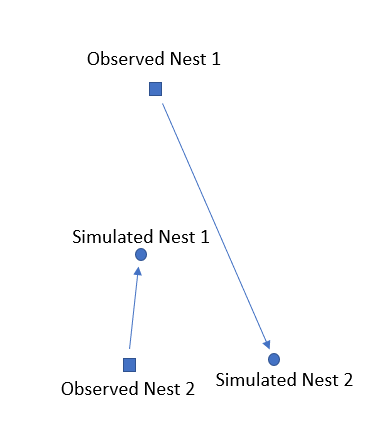
\includegraphics[width=0.3\linewidth]{subs1.PNG}}
 \subfloat[B]{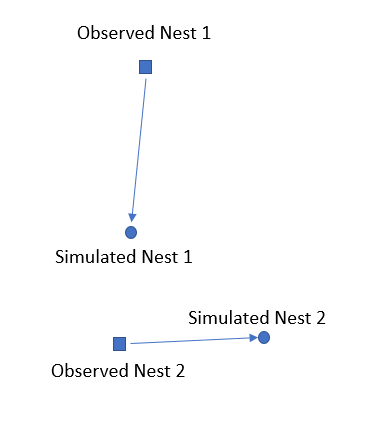
\includegraphics[width=0.3\linewidth]{subs2.PNG}}
\caption{[A] shows the shortest distance substitution in the deterministic scenario. [B] shows the more likely substitution that would be discarded in the deterministic scenario.}
\label{fig:1}
\end{figure*}

A better strategy is to assume that each particle can be corrected in a finite number of ways with probabilities $H_{Z^T}((\vec{s}^T)' | \vec{s}^T)$, where $(\vec{s}^T)'$ is the vector of the locations of the corrected nests at time $T$, which will depend on the distances between the simulated nests and the observations in the following way. Let us consider a simulated nest $s^T_i$ and an observation $z^T_j$. $s^T_i$ can be corrected by $z^T_j$ with probability $p_{ij} = p(s_i \leftrightarrow z_j) = e^{-d_{ij}}$ where $d_{ij}$ is the Euclidean distance between $s_i$ and $z_j$. Notice that when the distance is $d_{ij} = 0$ the probability $p_{ij}$ is 1 and the observation coincide with the simulated nest. The probability of a certain new configuration $k$ of nests will therefore be $p((\vec{s}^T)')_k = \prod p_{ij}$. The distribution of all the possible combinations will be $H_{Z^T} = \prod_k p((\vec{s}^T)')_k / \sum_k p((\vec{s}^T)')_k $. We then assume that each simulated particle can be corrected in only a finite number of ways to produce an element of the non-empty finite set $O_{\vec{z}^T} (\vec{s}^T)$ that contains all the allowed corrections. The correction is made selecting an element $(\vec{s}^T)'$ from $O_{\vec{z}^T} (\vec{s}^T)$ with probability $H_{Z^T} = \prod_k p((\vec{s}^T)')_k / \sum_k p((\vec{s}^T)')_k$.

The selected configuration for the corrections will also determine $T$ to be the time of observation for those nests that have been corrected. If a nests was simulated as unobserved at time $T$ we will correct also the time of observation

Note that we will correct only the nests that have not previously been corrected, so not all the possible combinations of substitutions will be explored.



This will introduce a term in the calculation of the weights in our sequential importance sampling approach.

\section{The Weights with non deterministic corrections}
}

\begin{thebibliography}{99}

\bibitem{Hawkes71} Hawkes A G (1971) Spectra of some self-exciting and mutually exciting point processes. \textit{Biometrika} 58(1): 83-90

\bibitem{Hawkes74} Hawkes A G, Oakes D (1974) A cluster Process Representation Of A Self-Exciting Point Process. \textit{Journal of Applied Probabilities} 11(3): 493-503

\bibitem{Keith} Keith J M, Spring D (2013) Agent-based Bayesian approach to monitoring the progress of invasive species eradication programs. \textit{Proc Natl Acad Sci} 110(33): 13428-13433

\bibitem{Jewell} Jewell C P, et al. (2009) Bayesian analysis for emerging infectious diseases. \textit{Bayesian Anal.} 4(3): 465-496

\bibitem{Lewis} Lewis P (1964) A Branching Poisson Process Model for the Analysis of Computer Failure Patterns. \textit{Journal of the Royal Statistical Society} 26(3): 398-456

\bibitem{Ogata} Ogata Y (1981) On Lewis' simulation method for point processes. \textit{IEEE Transactions on Information Theory} 27(1): 23-31

\bibitem{Reinhart} Reinhart A (2017) A review of self-exciting spatio-temporal point processes and their applications. \textit{ArXiv e-prints} 1708.02647v2

\bibitem{Shoenberg} Shoenberg F P, Brillinger R, Guttorp P (2014). Point Processes, Spatial Temporal. \textit{Encyclopedia of Environmetrics}

\bibitem{Zhuang} Zhuang J, Ogata Y, Vere-Jons D (204). Analyzing earthquake clustering features by using stochastic reconstruction. \textit{Journal Of Geophysical Research}

\end{thebibliography}


\end{document}
